\documentclass{beamer}
\usepackage{tikz}
\usetikzlibrary{shapes}
\usetheme{Madrid}

\tikzstyle{rec} = [rectangle,draw,text centered,minimum width={width("Application")+2pt}]

\title[CSE 300: UIS]{CSE 300: Presentation of User Interface System}
\author[1605113]{Md. Zunaed Karim (1605113)}
\institute[BUET]{Bangladesh University of Engineering and Technology}
\date{\today}

\begin{document}
	
	\begin{frame}{Equivalence Property}
		\begin{itemize}
			\item We can also define UIS as a function of series of interactions, $i_i$\\
			\item We call 2 UIS equivalent if for every possible input, they produce the same result
		\end{itemize}
	\end{frame}

	\begin{frame}{Properties of UIS using graphs}   	
	\begin{figure}[h]
    	\centering
    	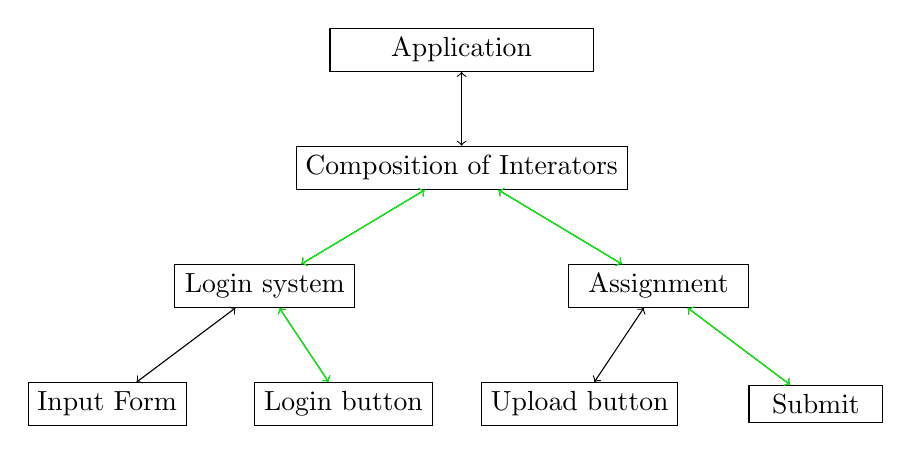
\begin{tikzpicture}
    	\node[rec,minimum width={width("Magnetometeraaaaaa")+2pt}](application) {Application};
    	
    	\node[rec,yshift=-0.5cm,minimum width={width("Magnetometeraaaaaa")+2pt},below of=application](composition) {Composition of Interators};
    	\draw[<->] (composition) -- (application);
    	
    	
    	\node[rec,xshift=-2.5cm,yshift=-0.5cm,minimum width={width("Magnetometer")+2pt},below of=composition](login) {Login system};
    	\draw[<->] (login) -- (composition);
    	
    	\node[rec,xshift=-2cm,yshift=-0.5cm,minimum width={width("Magnetom")+2pt},below of=login](form) {Input Form};
    	\draw[<->] (form) -- (login);
    	
    	\node[rec,xshift=2cm,minimum width={width("Magnetom")+2pt},right of=form](button) {Login button};
    	\draw[<->] (button) -- (login);
    	
    	
    	\node[rec,xshift=4cm,minimum width={width("Magnetometer")+2pt},right of=login](assignment) {Assignment};
    	\draw[<->] (assignment) -- (composition);
    	
    	
    	\node[rec,xshift=2cm,minimum width={width("Magnetom")+2pt},right of=button](upload) {Upload button};
    	\draw[<->] (upload) -- (assignment);
    	
    	\node[rec,xshift=2cm,minimum width={width("Magnetom")+2pt},right of=upload](submit) {Submit};
    	\draw[<->] (submit) -- (assignment);\pause
    	
    	\filldraw[green,<->] (submit) -- (assignment);\pause
    	\filldraw[green,<->] (assignment) -- (composition);\pause
		\filldraw[green,<->] (login) -- (composition);\pause
    	\filldraw[green,<->] (button) -- (login);
    	  	
    	\end{tikzpicture}
    \end{figure}
   	\end{frame}
   	
   	
	\begin{frame}{Properties of UIS using graphs}   	
	\begin{figure}[h]
    	\centering
    	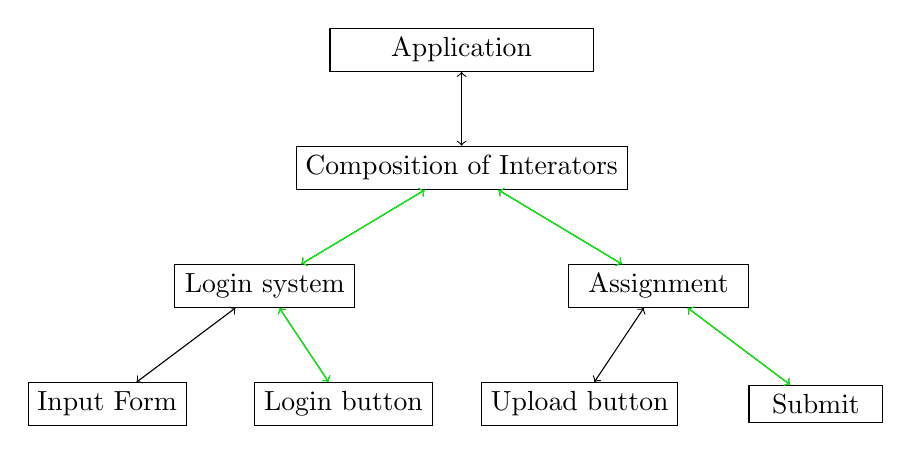
\begin{tikzpicture}
    	\node[rec,minimum width={width("Magnetometeraaaaaa")+2pt}](application) {Application};
    	
    	\node[rec,yshift=-0.5cm,minimum width={width("Magnetometeraaaaaa")+2pt},below of=application](composition) {Composition of Interators};
    	\draw[<->] (composition) -- (application);
    	
    	
    	\node[rec,xshift=-2.5cm,yshift=-0.5cm,minimum width={width("Magnetometer")+2pt},below of=composition](login) {Login system};
    	\draw[<->] (login) -- (composition);
    	
    	\node[rec,xshift=-2cm,yshift=-0.5cm,minimum width={width("Magnetom")+2pt},below of=login](form) {Input Form};
    	\draw[<->] (form) -- (login);
    	
    	\node[rec,xshift=2cm,minimum width={width("Magnetom")+2pt},right of=form](button) {Login button};
    	\draw[<->] (button) -- (login);
    	
    	
    	\node[rec,xshift=4cm,minimum width={width("Magnetometer")+2pt},right of=login](assignment) {Assignment};
    	\draw[<->] (assignment) -- (composition);
    	
    	
    	\node[rec,xshift=2cm,minimum width={width("Magnetom")+2pt},right of=button](upload) {Upload button};
    	\draw[<->] (upload) -- (assignment);
    	
    	\node[rec,xshift=2cm,minimum width={width("Magnetom")+2pt},right of=upload](submit) {Submit};
    	\draw[<->] (submit) -- (assignment);
    	
    	\filldraw[green,<->] (submit) -- (assignment);
    	\filldraw[green,<->] (assignment) -- (composition);
		\filldraw[green,<->] (login) -- (composition);
    	\filldraw[green,<->] (button) -- (login);

    	
    	  	
    	\end{tikzpicture}
    \end{figure}\pause
    
    \begin{itemize}
    	\item Communication consistency\pause
    	\item Connectivity property
    \end{itemize}
   	
   	\end{frame}
	
	\begin{frame}{Use of Properties}
		We can also use these properties to
	    \begin{itemize}
	    	\item Develop a precise model to identify redundancy and common mistakes in UIS design\pause
	    	\item Develop reusable libraries for UI design\pause
	    	\item Build automated tools for building and fixing UI
	    \end{itemize}
	\end{frame}
		
	
	
\end{document}